\section{System Design}
\begin{figure*}
    \centering
    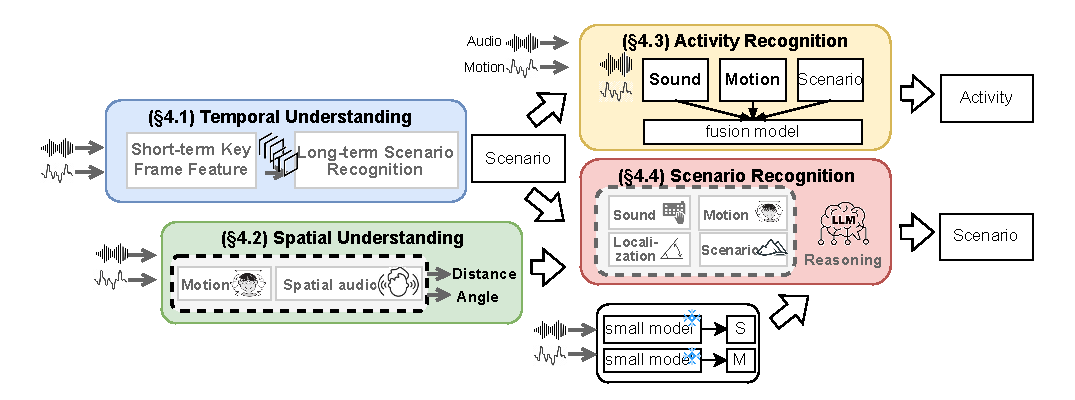
\includegraphics[width=0.8\linewidth]{chapters/egolog/figs/overview.pdf}
    \vspace{-1em}
      \caption{The system overview of EgoLog: the temporal and spatial understanding are two modules for multi-modal fusion, providing important input to the later modules to recognize activity and scenario}
      \vspace{-1em}
    \label{fig:egolog_system}
\end{figure*}

Figure~\ref{fig:egolog_system} provides an overview of EgoLog, a mobile system designed to capture egocentric daily logs over both long-term and short-term periods. 
Specifically, Section~\ref{sec:egolog_scenario} and Section~\ref{sec:egolog_localization} detail the fusion of audio and IMU data to achieve a deeper understanding of scenario (i.e., long-term descriptions) and spatial information (i.e., the relative location of sound sources). These insights serve as foundational clues for subsequent processing. 
In Section~\ref{sec:egolog_har}, we integrate the scenario information into the multi-modal activity recognition process, effectively mitigating modality collapse. Finally, Section~\ref{sec:egolog_llm} describes the use of an LLM as an expert to refine the scenario recognition from the previous stage; the resulting knowledge is subsequently transferred back to the local device.


\subsection{Temporal Understanding}
\label{sec:egolog_scenario}

\begin{figure}
  \centering
    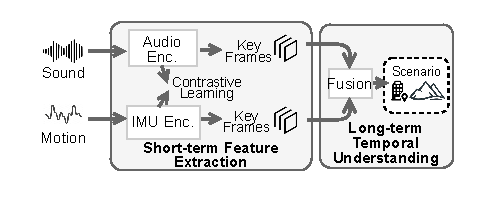
\includegraphics[width=1\linewidth]{chapters/egolog/figs/scenario.pdf}
    \vspace{-1em}
    \caption{Temporal understanding: we use contrastive learning to extract the cross-modal feature, which is important for the temporal-level fusion that recognize the scenario.}
    \vspace{-1em}
    \label{fig:egolog_scenario-recog}
\end{figure}

The measurement study indicates that recognizing many activities using IMU or audio data with an end-to-end model is difficult.
EgoLog therefore uses scenario recognition to provide prior information for activity recognition (Section~\ref{sec:egolog_har}). Scenario recognition also provides a useful high-level summary for daily logs.
As previously discussed, a scenario can be considered as a long-duration activity composed of multiple correlated sub-activities. To achieve accurate recognition, it is essential to develop an improved method for temporal analysis.
The pipeline is illustrated in Fig.~\ref{fig:egolog_scenario-recog}.


\subsubsection{Problem analysis}
Audio and IMU data have different properties and advantages. Their pretrained encoders are therefore optimized for different objectives. Simply merging their outputs may not produce the best results, as shown in Sec.~\ref{sec:egolog_measurement}; effective fusion must account for the heterogeneity of the two modalities.

We aim to tackle scenario recognition, which refers to identifying high-level human activities over an extended period (over 30 seconds). As detailed in Sec.~\ref{sec:egolog_measurement}, current pre-trained encoders already hold some scenario-level information, although they still fall short of ideal performance. A straightforward approach involves training a classification model using a dataset annotated with scenarios in an end-to-end fashion. Nonetheless, we have identified two persisting challenges: (1) the end-to-end model may struggle to generalize across different input lengths. (2) The performance might be inferior if scenarios are not included in the training data. Therefore, we propose training a new encoder for two modalities to obtain scenario-level features from brief time windows, which will then be applied in a secondary scenario recognition phase.

Given audio data and IMU data, the corresponding annotations for activity and scenario are assigned. Ideally, we could estimate activities individually and recognize scenarios accordingly. However, many activities may not relate to the audio or IMU data, such as silent motions that exceed the audio's capability.
Instead, we propose using two encoders: one for audio and one for IMU data. Their outputs would project the same feature space, representing features of the same scenario. Like activities, the two modalities may not always directly correlate with the scenario, so the mapping can fail sometimes. To address this, we can estimate the scenario by combining multiple windows of data, compensating for the sparsity of features.

\subsubsection{Contrastive learning}
Based on the preceding analysis, employing contrastive learning is optimal for capturing scenario-level features. Contrastive learning focuses on acquiring low-dimensional representations ($SE_i$) by differentiating between similar and dissimilar data samples. The method aims to group similar samples closely in the representation space while distancing dissimilar ones using the Euclidean distance. The efficacy of contrastive learning has been demonstrated in earlier research~\citep{han2023onellm, girdhar2023imagebind}. 
Within our framework, similarity and dissimilarity can be defined in two ways. Firstly, any data point aside from itself is deemed dissimilar. Secondly, data points within the same scenario are viewed as similar, whereas others are regarded as dissimilar. We expect that the first approach will yield more robust features, since it does not rely on explicit scenario annotations, and this will be assessed during the evaluation.

Regarding the network design, we employ two distinct deep neural networks to derive embeddings: LIMU-BERT~\citep{xu2021limu} for the IMU data and EfficientAT~\citep{lyu2024earda} for the audio input. Each sample spans a two-second window. The training of both encoders is based on the cross-entropy loss function, structured as follows:
\[
logits = (Audio_e \cdot IMU_e^T) \cdot \exp(\tau),
\]
where $Audio_e$ and $IMU_e$ refer to the features from two encoders, and $\tau$ refers to the learned temperature parameter \citep{chen2020simple}. Then, we get the loss using cross-entropy loss as follows:
\[
L = cross\_entropy\_loss(logits, label, axis=0).
\]

\subsubsection{Scenario recognition}
Assuming we extract the features from $Audio_e$ and $IMU_e$ by contrastive learning, they may not immediately convey the scenario as previously noted. We observe that a robust example in which both modalities relate to the scenario will exhibit a strong similarity between $Audio_e$ and $IMU_e$. This high similarity indicates that both modalities are effectively mapped into the same feature space, highlighting their importance as key features.
Conversely, low similarity suggests that the two modalities have not been successfully integrated into a unified representation of the scenario. Ideally, we would only keep frames with high similarity. However, the dynamics of execution can be problematic, introducing instability. Furthermore, it is difficult to set a definitive threshold to classify all frames below it as "useless."
Given the inherently weak correlation between audio and IMU, examples with high similarity may be rare. The model therefore needs to use as much information as possible from the available data.
To address this problem, we propose extending the key features along the temporal dimension. We integrate a sequence model—either an LSTM or a transformer—to compile features over time (as shown in the right section of Fig.~\ref{fig:egolog_scenario-recog}).
This two-stage architecture enables the model to capture both short-term and long-term dependencies within the features, thereby improving the accurate recognition of extended scenarios. Finally, a linear layer followed by a sigmoid activation function is used to predict the probability for each scenario.

\begin{figure}
  \centering
    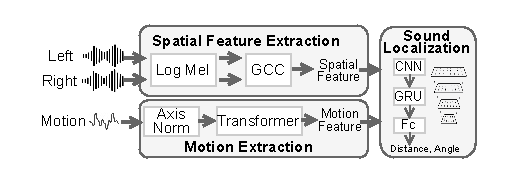
\includegraphics[width=1\linewidth]{chapters/egolog/figs/localization.pdf}
    \vspace{-1em}
    \caption{Spatial understanding: we differentiate sound by location by the combination of spatial audio and motion, leveraging the natural but random movement of the user.}
    \label{fig:egolog_seldnet}
    \vspace{-1em}
\end{figure}


\subsection{Spatial Understanding}
\label{sec:egolog_localization}
Existing activity recognition methods by audio are often misled by environmental events.
As illustrated in Sec. \ref{sec:egolog_measurement}, it is not enough to use sound volume to differentiate the near-field and far-field sound. Here, we are interested in the near-field sound because of the close correlation between it and the user's interaction with the environment. 

\subsubsection{Sound localization}
The location of sound can be estimated by a multi-channel microphone array. 
Specifically, the time of arrival of the sound source for one microphone is: \(t_i = \frac{\sqrt{(x_s - x_i)^2 + (y_s - y_i)^2}}{c}\), where the location of microphones $\mathbf{p}_i = (x_i, y_i)$, $i = 1, \ldots, N$, and a sound source at $\mathbf{s} = (x_s, y_s)$.
Since the start time of the sound source is unknown, the system can only obtain the time difference of arrival (TDoA) between two microphones, such as $i$ and $j$. With only two microphones on binaural earables, this yields a single equation, which is insufficient to resolve front--back confusion reliably.

Building on the work of SELDNet \citep{adavanne2018sound} and DeepEar \citep{yang2022deepear}, we propose a neural network-based binaural localization. Overall, our model performs an 8-class classification, distinguishing between four directions (front, left, right, back) and two distance categories (near and far). The binaural audio input, is converted to two log-Mel spectrograms and generalized cross-correlation coefficients of spectrograms, combined along the channel dimension to form spatial features with shape \( B \times 3 \times T \times 64 \), where \( B \) is the batch size and \( T \) is the number of frames. We process the audio feature with three convolutional layers, transforming it to (B, 128, T/5, 64). Then it is followed by a GRU layer, multi-head attention (resulting in B, 128, T/5, 64), and a linear layer that outputs (B, T/5, C).


\subsubsection{Movement compensation}

As illustrated in the motivation study, user movement can improve spatial understanding. Similar ideas have been used in prior work~\citep{zhu2021localizing, seo2022ross}, but these approaches require either explicit user gestures or a fully controllable robot. EgoLog instead uses natural, unintentional body movements that occur in daily life.

To realize this, we introduce an end-to-end method where IMU data—structured as (B, 6, T) and comprising both accelerometer and gyroscope measurements—is processed through two transformer layers. This module outputs a representation of shape (B, 384, T), which is then passed through a linear layer to produce an output of size (B, T/5, C). The resulting features are subsequently concatenated with the output from the GRU module.
The overall model performs an 8-class classification (C=8), distinguishing between four spatial directions (front, left, right, back) and two distance categories (near and far).

EgoLog cannot assume that only one sound source exists. Multiple sound sources may overlap, and both sound localization and audio recognition can be multi-label. This creates an association problem, which is addressed in a later section.

\subsection{Scenario-aware Activity Recognition}
\label{sec:egolog_har}

\begin{figure}
    \centering
    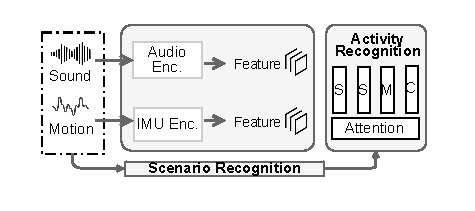
\includegraphics[width=1\linewidth]{chapters/egolog/figs/activity_recognition.pdf}
    \vspace{-1em}
    \caption{Multi-modal activity recognition: We extract features from each individual modality (uni-modal features), combine them with the scenario information derived from temporal understanding, and merge them at the token level for final activity recognition.}
    \vspace{-1em}
    \label{fig:egolog_activity_recognition}
\end{figure}

The methods outlined in Sec. \ref{sec:egolog_scenario} and \ref{sec:egolog_localization} offer a promising path for audio-IMU fusion. Next, we propose to integrate them into HAR.

Our proposed multi-modal network consists of two main components: unimodal backbones and a fusion module. The unimodal backbones include separate feature extractors that gather features from each input modality. The fusion module is designed to combine and aggregate these features from the unimodal backbones, resulting in a fused output that denotes the activity of the user. Although the design described above shows promise, it shares similar input and output characteristics with those presented in Section \ref{sec:egolog_measurement}, which has already been validated. As a result, it may not perform well in human activity recognition due to a lack of multi-modal correlation.

There are two common approaches for fusing modalities: using a multi-layer perceptron to process concatenated representations, or using a Transformer-based fusion module that processes a sequence of tokens from different modalities~\citep{gabeur2020multi}. EgoLog uses the Transformer-based design because attention can scale to a variable number of input tokens.
This flexibility is particularly important, as our multi-modal model needs to handle data with a varying number of modalities (more than only audio and IMU) for the task. Specifically, suppose the scenario information is a feature with the same dimension as other modalities, the transformer module can easily integrate it.
The final output of the fusion module is calculated by averaging the output tokens, rather than relying on the CLS token. The formulation of the token for one modality $Z_m$ is below:
\[
Z_m = (Encoder_m(S_m), e_m), \quad Z=f(Z_1, Z2, Z_3...)
\], where \( m \) represents each modality, which includes audio, IMU, and text. The term \( e_m \) denotes the learnable embedding specific to each modality. The transformer fusion module will combine multiple \( Z_m \) tokens and produce a unified \( Z \) feature with consistent dimensions. 
Similar to the previous section, we keep the audio and IMU encoder used for scenario recognition since both of them are lightweight and can be deployed on a mobile device.
By default, we use the standard transformer with a number of layers of 2. 

Next, we extend the multi-modal model that can handle not only the audio and IMU, but also other auxiliary information, such as scenario:
\begin{itemize}
    \item Specifically, we collect scenario information from Sec. \ref{sec:egolog_scenario} in textual form. To integrate it, we use the ImageBind \citep{girdhar2023imagebind} text encoder to map this information into the same feature space as the other modalities. Note that the text embeddings can be precomputed and stored to reduce computational overhead for each scenario. When multiple scenarios are detected, we concatenate their corresponding text representations.

    \item For spatial information from Sec. \ref{sec:egolog_localization}, we treat it as an indicator for interference detection. When far-field sound is detected with a confidence score exceeding 0.9, the audio recording is considered unreliable. In such cases, we can either discard the audio recording and rely solely on motion sensing or apply distance-based sound extraction \citep{chen2024hearable} to retain only the near-field sound.
\end{itemize} 


\subsection{LLM-assisted Scenario Recognition}
\label{sec:egolog_llm}
\begin{figure}
    \centering
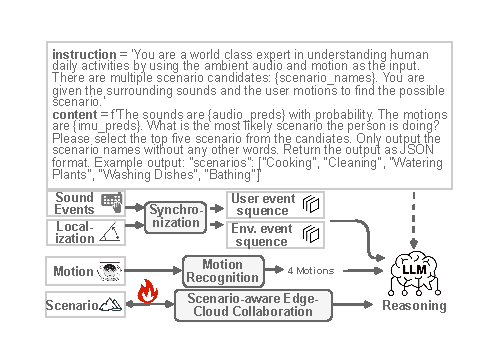
\includegraphics[width=1\linewidth]{chapters/egolog/figs/llm_reasoning.pdf}
\vspace{-2em}
    \caption{LLM-assisted scenario recognition: Utilizing prior outputs, we differentiate sound events into those originating from the user and those from the environment. We then combine it with motion and scenario recognition results and feed it into an LLM for reasoning (the upstream process). The LLM's output is then used as a pseudo-label to re-train the local model (the downstream process).}
    \vspace{-1em}
    \label{fig:egolog_llm_reasoning}
\end{figure}


As discussed in Section~\ref{sec:egolog_measurement}, LLMs may be suboptimal for direct activity recognition. They are better suited to higher-level scenario recognition, where longer data sequences provide richer context. This is consistent with Section~\ref{sec:egolog_scenario}, where longer sequences also benefit multimodal fusion. As illustrated in Fig.~\ref{fig:egolog_llm_reasoning}, EgoLog formats five-second sensor windows as text and uses tailored prompts to guide LLM-based scenario recognition. The LLM output can then refine local scenario predictions. All LLM processing is performed in the cloud so that the local EgoLog model remains lightweight.
 
\subsubsection{Prompt design}
Existing studies primarily use LLM reasoning on text-like data. This subsection introduces how EgoLog converts multimodal audio and motion signals into prompts for LLM-based scenario reasoning, as illustrated in Fig.~\ref{fig:egolog_llm_reasoning}. Instead of retraining the LLM or adding an adapter, EgoLog uses a specialized prompt with demonstrations that describe how to reason over sensor-derived context.
The prompt is structured as follows: “You are an expert in human activity analysis. You will receive audio and IMU recognition results, including extra information on potential scenarios. Using this information, reason and refine the person’s scenario. The scenario must be one of the following categories: [List of categories]. Your output must be a single line containing just one word or phrase.”
This prompt, along with the formatted input data as shown below, is fed to the LLM.

\paragraph{Audio.} 
We employ a pre-trained audio recognizer \citep{schmid2023efficient} to transcribe audio into text by selecting the top three predictions. The output is structured as "the detected audio classes are <class1, prob1>, <class2, prob2>, <class3, prob3>...", where each entry is referred to as a sound event. To minimize noise, we retain only the top five predictions with a confidence score exceeding 0.3.
Since the classifier's label set is based on the AudioSet ontology, the defined classes are highly fine-grained, often resulting in multiple similar classes with comparable probabilities. This lack of discriminative power hinders effective reasoning. To address this, we apply a two-level hierarchical clustering of the classes to their parent categories, reducing the total number of classes from 416 to 50 and improving generalization.

\paragraph{IMU.} 
Following the IMUCLIP approach \citep{moon2023imu2clip}, we classify IMU data into four activities: walking, moving, standing up, and sitting down. While previous works have demonstrated the ability to recognize more fine-grained activities using IMU data, their generalization capabilities remain questionable due to reliance on scenario-constrained datasets.

\paragraph{Spatial.}
EgoLog uses spatial information from Sec.~\ref{sec:egolog_localization} by applying different processing strategies to near-field and far-field audio inputs. For near-field sounds, the prompt states that the sound event occurs near the front of the user and is likely related to human activity. For far-field sounds, the prompt states that the sound event occurs at the estimated sound location.
When both near-field and far-field sounds are detected, it is unclear which event is near or far. As a result, we can turn on the distance-based sound separation \citep{chen2024hearable} that separate the audio into two and perform the sound recognition, respectively. We leave the optimization of the separation in the future work since it is unrelated to the main body of EgoLog.




\subsubsection{Scenario-aware LLM Assistance}

We define an upstream and downstream collaboration paradigm where the edge device seeks assistance from a cloud-based LLM, rather than naively querying the response.

For the upstream path, EgoLog uses the scenario recognition capability of LLMs, especially for out-of-domain data. The scenario estimated by the edge device is treated as a noisy reference that provides preliminary information to the LLM. The prompt includes this estimate and its confidence score.
Specifically, the estimated scenarios are added to the prompt, augmented by the text: "the preliminary scenario estimation is <scenario, confidence>."
However, frequent queries to the cloud service raise concerns about cost, privacy, and latency. Ideally, all modules of EgoLog should be executable on a mobile device if the performance is sufficient. Consequently, we propose a collaborative framework that strategically uses the cloud LLM to enhance the local model. Specifically, a confidence threshold (0.5) is set for the local scenario recognition model. A cloud query is triggered only when the local model's confidence is low.

Complementing the upstream process, we also propose a downstream collaboration where the cloud LLM's output can assist the local model. EgoLog sends the derived textual representation of an uncertain case, rather than its raw audio or IMU samples, to the LLM. The corresponding local sample and the LLM's refined label are then cached on the local device and used to fine-tune the local model, enabling continuous on-device improvement.
Within the scope of EgoLog, we do not consider adding new class to the local model since the required data can be huge, which leads to a long time for waiting.


